%% ENGR114_lab_assignment.tplx %%
%
% Built off of the article.tplx template %


% Default to the notebook output style

    


% Inherit from the specified cell style.




    
    \documentclass[11pt]{article}

    
    
    %% installed packages_rev2.tplx %%

\usepackage{fancyhdr}
\usepackage{lastpage}
\usepackage{framed,color}
\definecolor{shadecolor}{rgb}{.8,.8,.8}
\usepackage{titlesec}
% no indent on any paragraphs, vertical spacing between paragraphs is set to 1em
\usepackage[]{parskip}  % add [skip=1em] if the compiler will allow.

% for MATLAB syntax highlighting
\usepackage{listings}             % Include the listings-package
\definecolor{mygray}{rgb}{0.8,0.8,0.8} % color values Red, Green, Blue
\definecolor{mygreen}{RGB}{28,172,0}
\definecolor{mylilas}{RGB}{170,55,241}
    
    \usepackage[T1]{fontenc}
    % Nicer default font (+ math font) than Computer Modern for most use cases
    \usepackage{mathpazo}

    % Basic figure setup, for now with no caption control since it's done
    % automatically by Pandoc (which extracts ![](path) syntax from Markdown).
    \usepackage{graphicx}
    % We will generate all images so they have a width \maxwidth. This means
    % that they will get their normal width if they fit onto the page, but
    % are scaled down if they would overflow the margins.
    \makeatletter
    \def\maxwidth{\ifdim\Gin@nat@width>\linewidth\linewidth
    \else\Gin@nat@width\fi}
    \makeatother
    \let\Oldincludegraphics\includegraphics
    % Set max figure width to be 80% of text width, for now hardcoded.
    \renewcommand{\includegraphics}[1]{\Oldincludegraphics[width=.8\maxwidth]{#1}}
    % Ensure that by default, figures have no caption (until we provide a
    % proper Figure object with a Caption API and a way to capture that
    % in the conversion process - todo).
    \usepackage{caption}
    \DeclareCaptionLabelFormat{nolabel}{}
    \captionsetup{labelformat=nolabel}

    \usepackage{adjustbox} % Used to constrain images to a maximum size 
    \usepackage{xcolor} % Allow colors to be defined
    \usepackage{enumerate} % Needed for markdown enumerations to work
    \usepackage{geometry} % Used to adjust the document margins
    \usepackage{amsmath} % Equations
    \usepackage{amssymb} % Equations
    \usepackage{textcomp} % defines textquotesingle
    % Hack from http://tex.stackexchange.com/a/47451/13684:
    \AtBeginDocument{%
        \def\PYZsq{\textquotesingle}% Upright quotes in Pygmentized code
    }
    \usepackage{upquote} % Upright quotes for verbatim code
    \usepackage{eurosym} % defines \euro
    \usepackage[mathletters]{ucs} % Extended unicode (utf-8) support
    \usepackage[utf8x]{inputenc} % Allow utf-8 characters in the tex document
    \usepackage{fancyvrb} % verbatim replacement that allows latex
    \usepackage{grffile} % extends the file name processing of package graphics 
                         % to support a larger range 
    % The hyperref package gives us a pdf with properly built
    % internal navigation ('pdf bookmarks' for the table of contents,
    % internal cross-reference links, web links for URLs, etc.)
    \usepackage{hyperref}
    \usepackage{longtable} % longtable support required by pandoc >1.10
    \usepackage{booktabs}  % table support for pandoc > 1.12.2
    \usepackage[inline]{enumitem} % IRkernel/repr support (it uses the enumerate* environment)
    \usepackage[normalem]{ulem} % ulem is needed to support strikethroughs (\sout)
                                % normalem makes italics be italics, not underlines
    


    
    %% lab_title.tplx %% 
 
\newcommand{\labtitle}{Lab08 MicroPython} 
    %% header_and_footer.tplx %%

% Header and Footer
\lhead{\textbf{\labtitle}}
\rhead{ENGR114 Engineering Programming}
\lfoot{Portland Community College, \the\year}
\cfoot{}
\rfoot{\thepage~of~\pageref{LastPage}}  % must compile twice for LastPage

%lines below header and above footer
\renewcommand{\headrulewidth}{0.4pt}
\renewcommand{\footrulewidth}{0.4pt}

% Tabs
\newcommand{\itab}[1]{\hspace{0em}\rlap{#1}}
\newcommand{\tab}[1]{\hspace{.4\textwidth}\rlap{#1}}
\newcommand{\tabA}[1]{\hspace{.2\textwidth}\rlap{#1}}
    %% title_sec_formatting.tplx %%

\titleformat{\section}[block]{\LARGE\bfseries\filcenter}{}{1em}{}

\titleformat{\subsection}[hang]{\Large\bfseries}{}{1em}{}
\titlespacing{\subsection}{-1.4em}{1.5em}{1em}

\titleformat{\subsubsection}[hang]{\large\bfseries}{}{1em}{}
\titlespacing{\subsubsection}{-1.1em}{1.5em}{0.8em}
    
        \title{Problem Solving 101 with Python}
        \author{Peter D. Kazarinoff, PhD}
        \date{}
    
    
    
    % Colors for the hyperref package
    \definecolor{urlcolor}{rgb}{0,.145,.698}
    \definecolor{linkcolor}{rgb}{.71,0.21,0.01}
    \definecolor{citecolor}{rgb}{.12,.54,.11}

    % ANSI colors
    \definecolor{ansi-black}{HTML}{3E424D}
    \definecolor{ansi-black-intense}{HTML}{282C36}
    \definecolor{ansi-red}{HTML}{E75C58}
    \definecolor{ansi-red-intense}{HTML}{B22B31}
    \definecolor{ansi-green}{HTML}{00A250}
    \definecolor{ansi-green-intense}{HTML}{007427}
    \definecolor{ansi-yellow}{HTML}{DDB62B}
    \definecolor{ansi-yellow-intense}{HTML}{B27D12}
    \definecolor{ansi-blue}{HTML}{208FFB}
    \definecolor{ansi-blue-intense}{HTML}{0065CA}
    \definecolor{ansi-magenta}{HTML}{D160C4}
    \definecolor{ansi-magenta-intense}{HTML}{A03196}
    \definecolor{ansi-cyan}{HTML}{60C6C8}
    \definecolor{ansi-cyan-intense}{HTML}{258F8F}
    \definecolor{ansi-white}{HTML}{C5C1B4}
    \definecolor{ansi-white-intense}{HTML}{A1A6B2}

    % commands and environments needed by pandoc snippets
    % extracted from the output of `pandoc -s`
    \providecommand{\tightlist}{%
      \setlength{\itemsep}{0pt}\setlength{\parskip}{0pt}}
    \DefineVerbatimEnvironment{Highlighting}{Verbatim}{commandchars=\\\{\}}
    % Add ',fontsize=\small' for more characters per line
    \newenvironment{Shaded}{}{}
    \newcommand{\KeywordTok}[1]{\textcolor[rgb]{0.00,0.44,0.13}{\textbf{{#1}}}}
    \newcommand{\DataTypeTok}[1]{\textcolor[rgb]{0.56,0.13,0.00}{{#1}}}
    \newcommand{\DecValTok}[1]{\textcolor[rgb]{0.25,0.63,0.44}{{#1}}}
    \newcommand{\BaseNTok}[1]{\textcolor[rgb]{0.25,0.63,0.44}{{#1}}}
    \newcommand{\FloatTok}[1]{\textcolor[rgb]{0.25,0.63,0.44}{{#1}}}
    \newcommand{\CharTok}[1]{\textcolor[rgb]{0.25,0.44,0.63}{{#1}}}
    \newcommand{\StringTok}[1]{\textcolor[rgb]{0.25,0.44,0.63}{{#1}}}
    \newcommand{\CommentTok}[1]{\textcolor[rgb]{0.38,0.63,0.69}{\textit{{#1}}}}
    \newcommand{\OtherTok}[1]{\textcolor[rgb]{0.00,0.44,0.13}{{#1}}}
    \newcommand{\AlertTok}[1]{\textcolor[rgb]{1.00,0.00,0.00}{\textbf{{#1}}}}
    \newcommand{\FunctionTok}[1]{\textcolor[rgb]{0.02,0.16,0.49}{{#1}}}
    \newcommand{\RegionMarkerTok}[1]{{#1}}
    \newcommand{\ErrorTok}[1]{\textcolor[rgb]{1.00,0.00,0.00}{\textbf{{#1}}}}
    \newcommand{\NormalTok}[1]{{#1}}
    
    % Additional commands for more recent versions of Pandoc
    \newcommand{\ConstantTok}[1]{\textcolor[rgb]{0.53,0.00,0.00}{{#1}}}
    \newcommand{\SpecialCharTok}[1]{\textcolor[rgb]{0.25,0.44,0.63}{{#1}}}
    \newcommand{\VerbatimStringTok}[1]{\textcolor[rgb]{0.25,0.44,0.63}{{#1}}}
    \newcommand{\SpecialStringTok}[1]{\textcolor[rgb]{0.73,0.40,0.53}{{#1}}}
    \newcommand{\ImportTok}[1]{{#1}}
    \newcommand{\DocumentationTok}[1]{\textcolor[rgb]{0.73,0.13,0.13}{\textit{{#1}}}}
    \newcommand{\AnnotationTok}[1]{\textcolor[rgb]{0.38,0.63,0.69}{\textbf{\textit{{#1}}}}}
    \newcommand{\CommentVarTok}[1]{\textcolor[rgb]{0.38,0.63,0.69}{\textbf{\textit{{#1}}}}}
    \newcommand{\VariableTok}[1]{\textcolor[rgb]{0.10,0.09,0.49}{{#1}}}
    \newcommand{\ControlFlowTok}[1]{\textcolor[rgb]{0.00,0.44,0.13}{\textbf{{#1}}}}
    \newcommand{\OperatorTok}[1]{\textcolor[rgb]{0.40,0.40,0.40}{{#1}}}
    \newcommand{\BuiltInTok}[1]{{#1}}
    \newcommand{\ExtensionTok}[1]{{#1}}
    \newcommand{\PreprocessorTok}[1]{\textcolor[rgb]{0.74,0.48,0.00}{{#1}}}
    \newcommand{\AttributeTok}[1]{\textcolor[rgb]{0.49,0.56,0.16}{{#1}}}
    \newcommand{\InformationTok}[1]{\textcolor[rgb]{0.38,0.63,0.69}{\textbf{\textit{{#1}}}}}
    \newcommand{\WarningTok}[1]{\textcolor[rgb]{0.38,0.63,0.69}{\textbf{\textit{{#1}}}}}
    
    
    % Define a nice break command that doesn't care if a line doesn't already
    % exist.
    \def\br{\hspace*{\fill} \\* }
    % Math Jax compatability definitions
    \def\gt{>}
    \def\lt{<}
    % Document parameters
    
        \title{Problem Solving 101 with Python}
        \author{Peter D. Kazarinoff, PhD}
        \date{}
    
    
    
    

    % Pygments definitions
    
\makeatletter
\def\PY@reset{\let\PY@it=\relax \let\PY@bf=\relax%
    \let\PY@ul=\relax \let\PY@tc=\relax%
    \let\PY@bc=\relax \let\PY@ff=\relax}
\def\PY@tok#1{\csname PY@tok@#1\endcsname}
\def\PY@toks#1+{\ifx\relax#1\empty\else%
    \PY@tok{#1}\expandafter\PY@toks\fi}
\def\PY@do#1{\PY@bc{\PY@tc{\PY@ul{%
    \PY@it{\PY@bf{\PY@ff{#1}}}}}}}
\def\PY#1#2{\PY@reset\PY@toks#1+\relax+\PY@do{#2}}

\expandafter\def\csname PY@tok@w\endcsname{\def\PY@tc##1{\textcolor[rgb]{0.73,0.73,0.73}{##1}}}
\expandafter\def\csname PY@tok@c\endcsname{\let\PY@it=\textit\def\PY@tc##1{\textcolor[rgb]{0.25,0.50,0.50}{##1}}}
\expandafter\def\csname PY@tok@cp\endcsname{\def\PY@tc##1{\textcolor[rgb]{0.74,0.48,0.00}{##1}}}
\expandafter\def\csname PY@tok@k\endcsname{\let\PY@bf=\textbf\def\PY@tc##1{\textcolor[rgb]{0.00,0.50,0.00}{##1}}}
\expandafter\def\csname PY@tok@kp\endcsname{\def\PY@tc##1{\textcolor[rgb]{0.00,0.50,0.00}{##1}}}
\expandafter\def\csname PY@tok@kt\endcsname{\def\PY@tc##1{\textcolor[rgb]{0.69,0.00,0.25}{##1}}}
\expandafter\def\csname PY@tok@o\endcsname{\def\PY@tc##1{\textcolor[rgb]{0.40,0.40,0.40}{##1}}}
\expandafter\def\csname PY@tok@ow\endcsname{\let\PY@bf=\textbf\def\PY@tc##1{\textcolor[rgb]{0.67,0.13,1.00}{##1}}}
\expandafter\def\csname PY@tok@nb\endcsname{\def\PY@tc##1{\textcolor[rgb]{0.00,0.50,0.00}{##1}}}
\expandafter\def\csname PY@tok@nf\endcsname{\def\PY@tc##1{\textcolor[rgb]{0.00,0.00,1.00}{##1}}}
\expandafter\def\csname PY@tok@nc\endcsname{\let\PY@bf=\textbf\def\PY@tc##1{\textcolor[rgb]{0.00,0.00,1.00}{##1}}}
\expandafter\def\csname PY@tok@nn\endcsname{\let\PY@bf=\textbf\def\PY@tc##1{\textcolor[rgb]{0.00,0.00,1.00}{##1}}}
\expandafter\def\csname PY@tok@ne\endcsname{\let\PY@bf=\textbf\def\PY@tc##1{\textcolor[rgb]{0.82,0.25,0.23}{##1}}}
\expandafter\def\csname PY@tok@nv\endcsname{\def\PY@tc##1{\textcolor[rgb]{0.10,0.09,0.49}{##1}}}
\expandafter\def\csname PY@tok@no\endcsname{\def\PY@tc##1{\textcolor[rgb]{0.53,0.00,0.00}{##1}}}
\expandafter\def\csname PY@tok@nl\endcsname{\def\PY@tc##1{\textcolor[rgb]{0.63,0.63,0.00}{##1}}}
\expandafter\def\csname PY@tok@ni\endcsname{\let\PY@bf=\textbf\def\PY@tc##1{\textcolor[rgb]{0.60,0.60,0.60}{##1}}}
\expandafter\def\csname PY@tok@na\endcsname{\def\PY@tc##1{\textcolor[rgb]{0.49,0.56,0.16}{##1}}}
\expandafter\def\csname PY@tok@nt\endcsname{\let\PY@bf=\textbf\def\PY@tc##1{\textcolor[rgb]{0.00,0.50,0.00}{##1}}}
\expandafter\def\csname PY@tok@nd\endcsname{\def\PY@tc##1{\textcolor[rgb]{0.67,0.13,1.00}{##1}}}
\expandafter\def\csname PY@tok@s\endcsname{\def\PY@tc##1{\textcolor[rgb]{0.73,0.13,0.13}{##1}}}
\expandafter\def\csname PY@tok@sd\endcsname{\let\PY@it=\textit\def\PY@tc##1{\textcolor[rgb]{0.73,0.13,0.13}{##1}}}
\expandafter\def\csname PY@tok@si\endcsname{\let\PY@bf=\textbf\def\PY@tc##1{\textcolor[rgb]{0.73,0.40,0.53}{##1}}}
\expandafter\def\csname PY@tok@se\endcsname{\let\PY@bf=\textbf\def\PY@tc##1{\textcolor[rgb]{0.73,0.40,0.13}{##1}}}
\expandafter\def\csname PY@tok@sr\endcsname{\def\PY@tc##1{\textcolor[rgb]{0.73,0.40,0.53}{##1}}}
\expandafter\def\csname PY@tok@ss\endcsname{\def\PY@tc##1{\textcolor[rgb]{0.10,0.09,0.49}{##1}}}
\expandafter\def\csname PY@tok@sx\endcsname{\def\PY@tc##1{\textcolor[rgb]{0.00,0.50,0.00}{##1}}}
\expandafter\def\csname PY@tok@m\endcsname{\def\PY@tc##1{\textcolor[rgb]{0.40,0.40,0.40}{##1}}}
\expandafter\def\csname PY@tok@gh\endcsname{\let\PY@bf=\textbf\def\PY@tc##1{\textcolor[rgb]{0.00,0.00,0.50}{##1}}}
\expandafter\def\csname PY@tok@gu\endcsname{\let\PY@bf=\textbf\def\PY@tc##1{\textcolor[rgb]{0.50,0.00,0.50}{##1}}}
\expandafter\def\csname PY@tok@gd\endcsname{\def\PY@tc##1{\textcolor[rgb]{0.63,0.00,0.00}{##1}}}
\expandafter\def\csname PY@tok@gi\endcsname{\def\PY@tc##1{\textcolor[rgb]{0.00,0.63,0.00}{##1}}}
\expandafter\def\csname PY@tok@gr\endcsname{\def\PY@tc##1{\textcolor[rgb]{1.00,0.00,0.00}{##1}}}
\expandafter\def\csname PY@tok@ge\endcsname{\let\PY@it=\textit}
\expandafter\def\csname PY@tok@gs\endcsname{\let\PY@bf=\textbf}
\expandafter\def\csname PY@tok@gp\endcsname{\let\PY@bf=\textbf\def\PY@tc##1{\textcolor[rgb]{0.00,0.00,0.50}{##1}}}
\expandafter\def\csname PY@tok@go\endcsname{\def\PY@tc##1{\textcolor[rgb]{0.53,0.53,0.53}{##1}}}
\expandafter\def\csname PY@tok@gt\endcsname{\def\PY@tc##1{\textcolor[rgb]{0.00,0.27,0.87}{##1}}}
\expandafter\def\csname PY@tok@err\endcsname{\def\PY@bc##1{\setlength{\fboxsep}{0pt}\fcolorbox[rgb]{1.00,0.00,0.00}{1,1,1}{\strut ##1}}}
\expandafter\def\csname PY@tok@kc\endcsname{\let\PY@bf=\textbf\def\PY@tc##1{\textcolor[rgb]{0.00,0.50,0.00}{##1}}}
\expandafter\def\csname PY@tok@kd\endcsname{\let\PY@bf=\textbf\def\PY@tc##1{\textcolor[rgb]{0.00,0.50,0.00}{##1}}}
\expandafter\def\csname PY@tok@kn\endcsname{\let\PY@bf=\textbf\def\PY@tc##1{\textcolor[rgb]{0.00,0.50,0.00}{##1}}}
\expandafter\def\csname PY@tok@kr\endcsname{\let\PY@bf=\textbf\def\PY@tc##1{\textcolor[rgb]{0.00,0.50,0.00}{##1}}}
\expandafter\def\csname PY@tok@bp\endcsname{\def\PY@tc##1{\textcolor[rgb]{0.00,0.50,0.00}{##1}}}
\expandafter\def\csname PY@tok@fm\endcsname{\def\PY@tc##1{\textcolor[rgb]{0.00,0.00,1.00}{##1}}}
\expandafter\def\csname PY@tok@vc\endcsname{\def\PY@tc##1{\textcolor[rgb]{0.10,0.09,0.49}{##1}}}
\expandafter\def\csname PY@tok@vg\endcsname{\def\PY@tc##1{\textcolor[rgb]{0.10,0.09,0.49}{##1}}}
\expandafter\def\csname PY@tok@vi\endcsname{\def\PY@tc##1{\textcolor[rgb]{0.10,0.09,0.49}{##1}}}
\expandafter\def\csname PY@tok@vm\endcsname{\def\PY@tc##1{\textcolor[rgb]{0.10,0.09,0.49}{##1}}}
\expandafter\def\csname PY@tok@sa\endcsname{\def\PY@tc##1{\textcolor[rgb]{0.73,0.13,0.13}{##1}}}
\expandafter\def\csname PY@tok@sb\endcsname{\def\PY@tc##1{\textcolor[rgb]{0.73,0.13,0.13}{##1}}}
\expandafter\def\csname PY@tok@sc\endcsname{\def\PY@tc##1{\textcolor[rgb]{0.73,0.13,0.13}{##1}}}
\expandafter\def\csname PY@tok@dl\endcsname{\def\PY@tc##1{\textcolor[rgb]{0.73,0.13,0.13}{##1}}}
\expandafter\def\csname PY@tok@s2\endcsname{\def\PY@tc##1{\textcolor[rgb]{0.73,0.13,0.13}{##1}}}
\expandafter\def\csname PY@tok@sh\endcsname{\def\PY@tc##1{\textcolor[rgb]{0.73,0.13,0.13}{##1}}}
\expandafter\def\csname PY@tok@s1\endcsname{\def\PY@tc##1{\textcolor[rgb]{0.73,0.13,0.13}{##1}}}
\expandafter\def\csname PY@tok@mb\endcsname{\def\PY@tc##1{\textcolor[rgb]{0.40,0.40,0.40}{##1}}}
\expandafter\def\csname PY@tok@mf\endcsname{\def\PY@tc##1{\textcolor[rgb]{0.40,0.40,0.40}{##1}}}
\expandafter\def\csname PY@tok@mh\endcsname{\def\PY@tc##1{\textcolor[rgb]{0.40,0.40,0.40}{##1}}}
\expandafter\def\csname PY@tok@mi\endcsname{\def\PY@tc##1{\textcolor[rgb]{0.40,0.40,0.40}{##1}}}
\expandafter\def\csname PY@tok@il\endcsname{\def\PY@tc##1{\textcolor[rgb]{0.40,0.40,0.40}{##1}}}
\expandafter\def\csname PY@tok@mo\endcsname{\def\PY@tc##1{\textcolor[rgb]{0.40,0.40,0.40}{##1}}}
\expandafter\def\csname PY@tok@ch\endcsname{\let\PY@it=\textit\def\PY@tc##1{\textcolor[rgb]{0.25,0.50,0.50}{##1}}}
\expandafter\def\csname PY@tok@cm\endcsname{\let\PY@it=\textit\def\PY@tc##1{\textcolor[rgb]{0.25,0.50,0.50}{##1}}}
\expandafter\def\csname PY@tok@cpf\endcsname{\let\PY@it=\textit\def\PY@tc##1{\textcolor[rgb]{0.25,0.50,0.50}{##1}}}
\expandafter\def\csname PY@tok@c1\endcsname{\let\PY@it=\textit\def\PY@tc##1{\textcolor[rgb]{0.25,0.50,0.50}{##1}}}
\expandafter\def\csname PY@tok@cs\endcsname{\let\PY@it=\textit\def\PY@tc##1{\textcolor[rgb]{0.25,0.50,0.50}{##1}}}

\def\PYZbs{\char`\\}
\def\PYZus{\char`\_}
\def\PYZob{\char`\{}
\def\PYZcb{\char`\}}
\def\PYZca{\char`\^}
\def\PYZam{\char`\&}
\def\PYZlt{\char`\<}
\def\PYZgt{\char`\>}
\def\PYZsh{\char`\#}
\def\PYZpc{\char`\%}
\def\PYZdl{\char`\$}
\def\PYZhy{\char`\-}
\def\PYZsq{\char`\'}
\def\PYZdq{\char`\"}
\def\PYZti{\char`\~}
% for compatibility with earlier versions
\def\PYZat{@}
\def\PYZlb{[}
\def\PYZrb{]}
\makeatother


    % Exact colors from NB
    \definecolor{incolor}{rgb}{0.0, 0.0, 0.5}
    \definecolor{outcolor}{rgb}{0.545, 0.0, 0.0}




    
    % Prevent overflowing lines due to hard-to-break entities
    \sloppy 
    % Setup hyperref package
    \hypersetup{
      breaklinks=true,  % so long urls are correctly broken across lines
      colorlinks=true,
      urlcolor=urlcolor,
      linkcolor=linkcolor,
      citecolor=citecolor,
      }
    % Slightly bigger margins than the latex defaults
    
    %% margins.tplx %%

% margins
\textwidth=7in
\textheight=9.0in
\topmargin=-0.5in
\headheight=15pt
\headsep=.5in
\hoffset = -0.5in

\pagestyle{fancy}

    

    \begin{document}
    
    
    

    
    

    
    \hypertarget{lab-08---micropython}{%
\section{Lab 08 - MicroPython}\label{lab-08---micropython}}

    \href{http://micropython.org/}{MicroPython} is a port, or version of
Python designed to run on small, inexpensive, low-power
microcontrollers. Traditionally, Python is run on a desktop or laptop
computer (also on cloud servers). Compared to a desktop or laptop,
microcontrollers are much smaller, cheaper and less powerful. A
``regular'' version of Python can't run on small, cheap microcontrollers
because Python is too resource intensive. Regular Python takes up too
much hard disk space, runs on too much RAM and requires a more powerful
processor than microcontrollers have.

To get MicroPython to run at all on these small microcontroller boards,
MicroPython only contains a subset of all the standard library modules
included with ``regular'' Python. Some of the libraries that are
included with MicroPython don't have the full set of functions and
classes that come with the full version of Python. This limited
functionality allows MicroPython to be compact (around 600 kB for the
ESP8266 port) and only use a small amount of RAM (down to 16k according
to the \href{https://micropython.org/}{Micropython main page}.)

    \hypertarget{prelab}{%
\subsection{Prelab}\label{prelab}}

Before you start the lab, try using the MicroPython online with a
broswer-based \href{https://micropython.org/unicorn/}{MicroPython online
emulator}. The emulator allows you to run commands at a MicroPython
Prompt and see the result on a virtual pyboard.

Also browse through the
\href{https://docs.micropython.org/en/latest/}{MicroPython Docs} and in
particular the
\href{https://docs.micropython.org/en/latest/esp8266/quickref.html}{ESP8266}
section. You will use an ESP8266-based microcontroller in this lab.

    \hypertarget{lab}{%
\subsection{Lab}\label{lab}}

    \hypertarget{installation}{%
\subsubsection{Installation}\label{installation}}

MicroPython should already be installed on your ESP8266 Microcontroller
when you start the lab. If you are unable to run any commands at the
MicroPython REPL, this might mean that MicroPython has not been
pre-installed. Check with your instructor to determine if MicorPython
installation is the issue. If you do need to install MicroPython on your
ESP8266, refer to this resource:
\href{https://pythonforundergradengineers.com/micropython-install.html}{Installing
Micropython on an Adafruit Feather Huzzah ESP8266}

    \hypertarget{connect-the-esp8266-microcontroller-to-your-computer}{%
\subsubsection{Connect the ESP8266 microcontroller to your
computer}\label{connect-the-esp8266-microcontroller-to-your-computer}}

    Use a microUSB cable to connect the microcontroller to the computer.
Make sure that the microUSB cable is a full USB data cable and not just
a simple power cable. Cables that are just used to charge phones may
only be power cables and may not be capable of transmitting data. The
cable you are provided with in lab is a microUSB data cable and should
work.

    \hypertarget{determine-which-serial-port-the-esp8266-microcontroller-is-connected-to}{%
\subsubsection{Determine which serial port the ESP8266 microcontroller
is connected
to}\label{determine-which-serial-port-the-esp8266-microcontroller-is-connected-to}}

    Use Windows Device Manager to determine which serial port the Feather
Huzzah is connected to. O Windows 10, the microcontroller usually comes
up as \texttt{COM4}. You can find the serial port by looking in the
Ports (COM \& LPT) category of the Windows Device Manager. Look for
something like \textbf{Silicon Labs CP210x USB to UART Bridge (COM4)} in
the \textbf{Ports (COM \& LPT)} menu. It is the \textbf{COM\#} that you
are looking for.

\begin{figure}
\centering
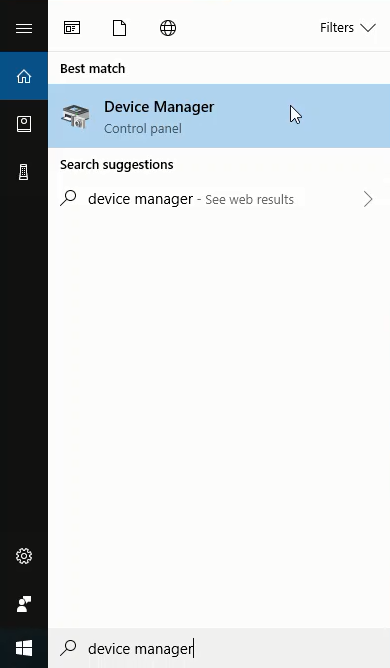
\includegraphics{images/find_device_manager.png}
\caption{Find the Windows 10 Device Manager}
\end{figure}

\begin{figure}
\centering
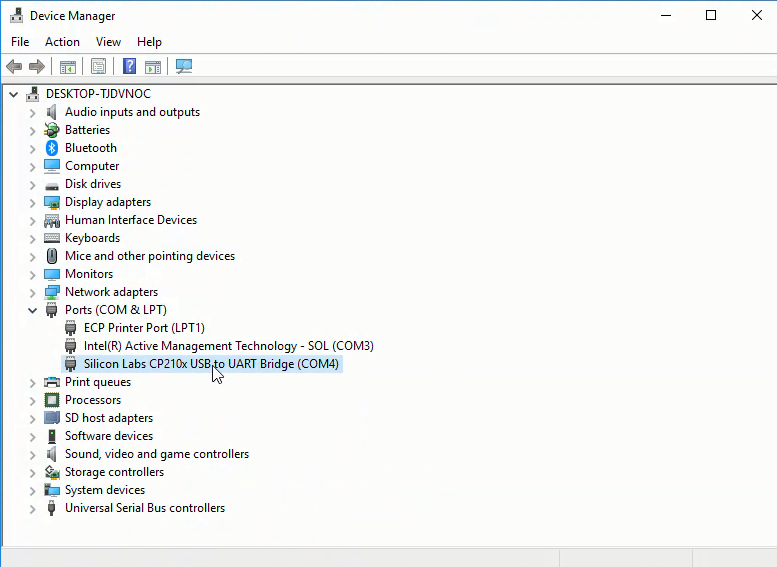
\includegraphics{images/device_manager_menu.png}
\caption{Device Manager Menu on Windows 10}
\end{figure}

    \hypertarget{use-putty-to-connect-to-the-esp8266-microcontroller}{%
\subsubsection{Use PuTTY to connect to the ESP8266
microcontroller}\label{use-putty-to-connect-to-the-esp8266-microcontroller}}

    Ensure the ESP8266 board is connected with a USB cable, then connect to
it with a program called PuTTY. Set the proper serial port (COM\#) and
and specify 115200 baud. Remember to use the \textbf{Serial} radio
button under \textbf{Connection Type:} to select serial communication or
you will be trying to communicate with the ESP8266 Microcontroller over
SSH which won't work.

\begin{figure}
\centering
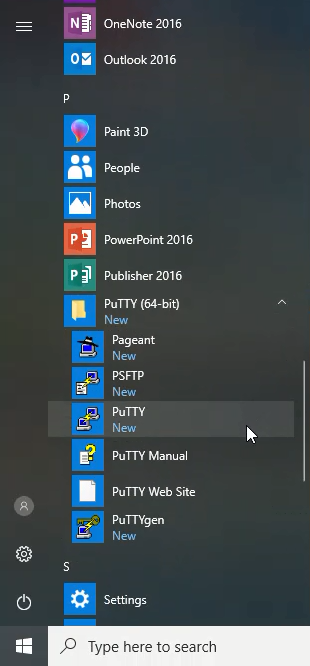
\includegraphics{images/putty_in_start_menu.png}
\caption{PuTTY in Windows 10 start menu}
\end{figure}

\begin{figure}
\centering
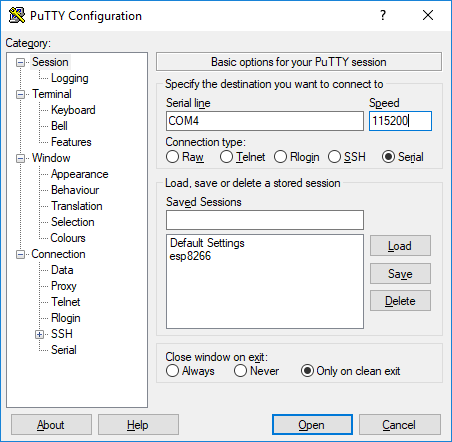
\includegraphics{images/putty_config.PNG}
\caption{PuTTY configuration}
\end{figure}

This should bring up the MicroPython REPL prompt
\texttt{\textgreater{}\textgreater{}\textgreater{}}. If you can't see
the \texttt{\textgreater{}\textgreater{}\textgreater{}} prompt, try
typing {[}Enter{]}, Ctrl-D, pushing the RESET button on the ESP8266
microcontroller or unplugging then replugging the USB cable.

\begin{figure}
\centering
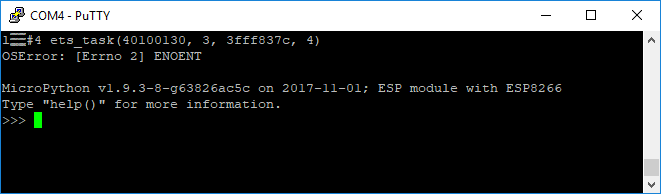
\includegraphics{images/REPL_prompt.PNG}
\caption{MicroPython REPL prompt}
\end{figure}

    \hypertarget{run-commands-at-the-prompt-to-turn-the-built-in-led-on-the-adafruit-feather-huzzah-esp8266-on-and-off}{%
\subsubsection{Run commands at the prompt to turn the built-in LED on
the Adafruit Feather Huzzah ESP8266 on and
off}\label{run-commands-at-the-prompt-to-turn-the-built-in-led-on-the-adafruit-feather-huzzah-esp8266-on-and-off}}

    At the MicroPython REPL (the MicroPython command prompt
\texttt{\textgreater{}\textgreater{}\textgreater{}}) try the following
commands:

\begin{verbatim}
>>> print('MicroPython for Engineers!')
MicroPython for Engineers
\end{verbatim}

If we import the \texttt{sys} module, we can see the MicroPython
implementation and platform.

\begin{verbatim}
>>> import sys
>>> sys.implementation
(name='micropython', version=(1, 9, 3))
>>> sys.platform
'esp8266'
\end{verbatim}

\begin{figure}
\centering
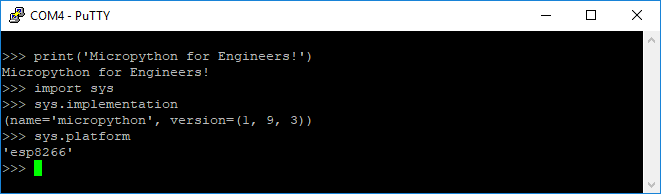
\includegraphics{images/sys_dot_implementation_and_platform.PNG}
\caption{Results of running sys commands at the MicroPython REPL prompt}
\end{figure}

If you see similar output, that means MicroPython is working on the
ESP8266 Microcontroller. We can also view the flash memory size of our
microcontroller and the size of the MicroPython firmware we installed.
Try this at the MicroPython prompt:

\begin{verbatim}
>>> import port_diag
\end{verbatim}

\begin{figure}
\centering
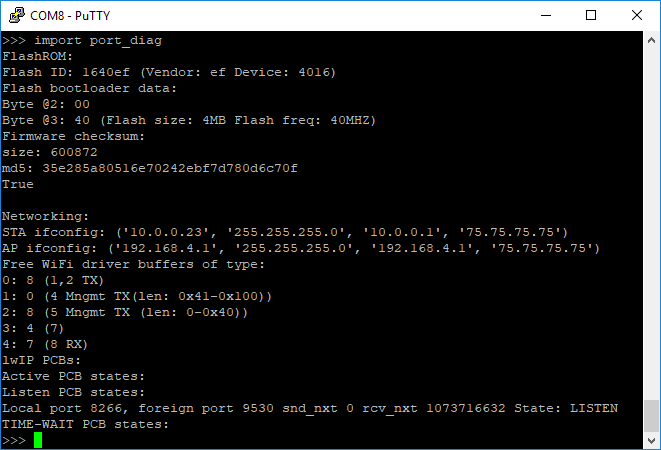
\includegraphics{images/import_port_diag.PNG}
\caption{Results of running import port\_diag at the MicroPython REPL
prompt}
\end{figure}

We can see the flash memory size is 4 MB. Below the label
\texttt{Firmware\ checksum:} we can see a line for
\texttt{size:\ 600872}. This means the size of our Micropythpon
installation is about 600 KB or 0.6 MB. Just over half a megabyte and we
are running a working version of Python!

    \hypertarget{blinking-a-led}{%
\subsection{Blinking a LED}\label{blinking-a-led}}

    The ESP8266 microcontroller as a built-in red LED mounted on the board
close to the USB cable input. MicroPython can be used to blink this LED
on and off.

    Connect an LED to the ESP8266 Microcontroller as shown below.

\begin{itemize}
\tightlist
\item
  Connect Pin 13 to the LONG leg of the LED (red wire)
\item
  Connect GND to the SHORT leg of the LED to through a 330 \(\Omega\)
  resistor (black wire).
\end{itemize}

\begin{figure}
\centering
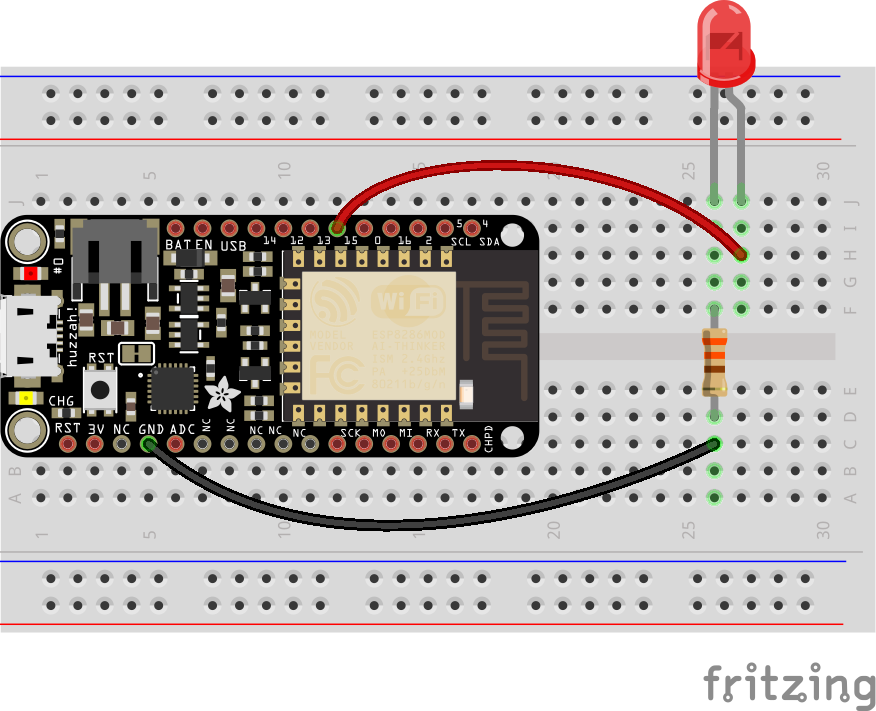
\includegraphics{images/feather_huzzah_LED_bb.png}
\caption{fritzing diagram ESP8266 LED}
\end{figure}

    In the PuTTY serial window, test to see if the MicroPython REPL is still
functioning with a basic \emph{Hello World} program.

\begin{verbatim}
>>> print("Hello World")
Hello World
\end{verbatim}

Next, we will blink the ESP8266 micrcontroller's built-in LED. The
microcontroller has a built-in LED connected to Pin 0. If we control the
current going to Pin 0, we control the built-in LED. To control a Pin
using MicroPython, first import the \textbf{machine} module. Next a
\texttt{Pin} object needs to be created. The integer passed into
\texttt{machine.Pin()} determines the pin number assigned to the
\texttt{Pin} object.

\begin{verbatim}
>>> import machine
>>> pin = machine.Pin(0)
\end{verbatim}

The value (on or off) of Pin 0 can be returned using

\begin{verbatim}
>>> pin.value
1
\end{verbatim}

To assign a value to Pin 0, the \texttt{Pin} object must be created as
an \emph{output} pin. An output pin is a pin where a program or user
determines the pin output. An input pin is a pin set up to read input,
like the input from a sensor. In this case we want to assign Pin 0 as an
output pin.

\begin{verbatim}
>>> pin = machine.Pin(0, machine.Pin.OUT)

# turn the LED on
>>> pin.value(0)

# turn the LED off
>>> pin.value(1)
\end{verbatim}

    \hypertarget{run-code-at-the-micropython-repl-to-blink-the-led}{%
\subsubsection{Run code at the MicroPython REPL to blink the
LED}\label{run-code-at-the-micropython-repl-to-blink-the-led}}

    Now we can write a for loop at the MicroPython REPL to blink the LED on
and off. In order to do this, we need to import the \textbf{machine}
module and the \textbf{time} module.

    \begin{verbatim}
>>> import machine
>>> import time
>>> pin = machine.Pin(0, machine.Pin.OUT)
>>> for i in range(10):
...     pin.value(1)
...     time.sleep(0.5)
...     pin.value(0)
...     time.sleep(0.5)
# backspace to exit loop indent and execute the loop.
.... 
\end{verbatim}

    \hypertarget{reading-a-potentiometer}{%
\subsection{Reading a potentiometer}\label{reading-a-potentiometer}}

    In this section, you will learn how to connect a potentiometer sensor to
the ESP8266 Microcontroller and use the MicroPython REPL to record the
potentiometer level.

    \hypertarget{connect-the-potentiometer-to-the-esp8266-microcontroller}{%
\subsubsection{Connect the potentiometer to the ESP8266
Microcontroller}\label{connect-the-potentiometer-to-the-esp8266-microcontroller}}

Connect the potentiometer to the ESP8266 Microcontroller as shown below.
Connect Pin 13 to the LONG leg of the LED (red wire) and connect the
SHORT leg of the LED to ground through a 330 \(\Omega\) resistor (black
wire).

\begin{figure}
\centering
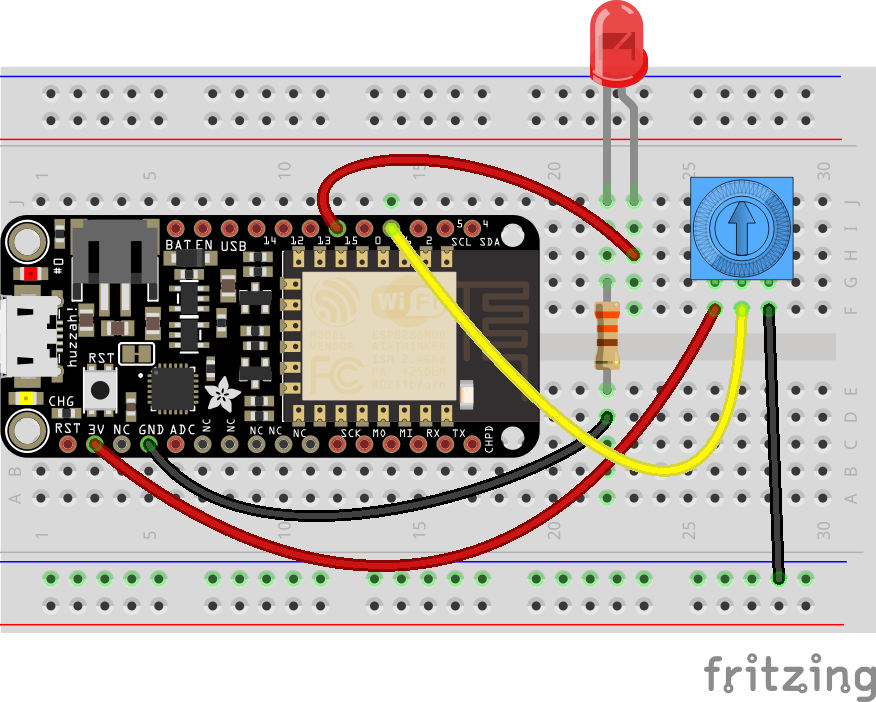
\includegraphics{images/feather_huzzah_potentiometer_bb.png}
\caption{fritzing diagram ESP8266 LED}
\end{figure}

    \hypertarget{run-code-at-the-micropython-repl-to-measure-the-light-level}{%
\subsubsection{Run code at the MicroPython REPL to measure the light
level}\label{run-code-at-the-micropython-repl-to-measure-the-light-level}}

    In the PuTTY serial window, import the \texttt{machine} module and then
create an instance of the \texttt{machine.I2C} class with the
\texttt{scl} and \texttt{sda} parameters set as
\texttt{scl=machine.Pin(5)} and \texttt{sda=machine.Pin(4)}. Then create
an empty \texttt{bytearray} which will store the data coming in from the
MCP9808 temperature sensor. As strings in Micropython are UTF-8 encoded
by default (like in Python 3), a \emph{bytearray} needs to be used to
read the raw output from the MCP9808 chip registers. The command
\texttt{i2c.readfrom\_mem\_into()} method brings in the data from the
sensor and saves it to the \texttt{byte\_data} variable. The arguments
inside the \texttt{i2c.readfrom\_mem\_into()} method \texttt{24} and
\texttt{5} correspond to the I2C memory address and registry address of
the temperature data stored in the MCP9808 temperature sensor.

\begin{verbatim}
>>> import machine
>>> import time
>>> pin = machine.Pin(0, machine.Pin.IN)
>>> for i in range(10):
...     print(pin.value())
...     time.sleep(0.5)
# backspace to exit loop indent and execute the loop.
.... 
\end{verbatim}

    \hypertarget{deliverables}{%
\subsection{Deliverables}\label{deliverables}}

Before closing the PuTTY window, run the command \texttt{history}. Copy
the ouput from the window into a text file. Save the file as
\texttt{lab8.txt}. Upload the \texttt{lab8.tct} file to D2L.

    \hypertarget{by-p.-kazarinoff-portland-community-college-2018}{%
\paragraph{\texorpdfstring{\emph{By P. Kazarinoff, Portland Community
College,
2018}}{By P. Kazarinoff, Portland Community College, 2018}}\label{by-p.-kazarinoff-portland-community-college-2018}}


    % Add a bibliography block to the postdoc
    
    
    
    \end{document}
